\begin{figure}[ht]
\centering
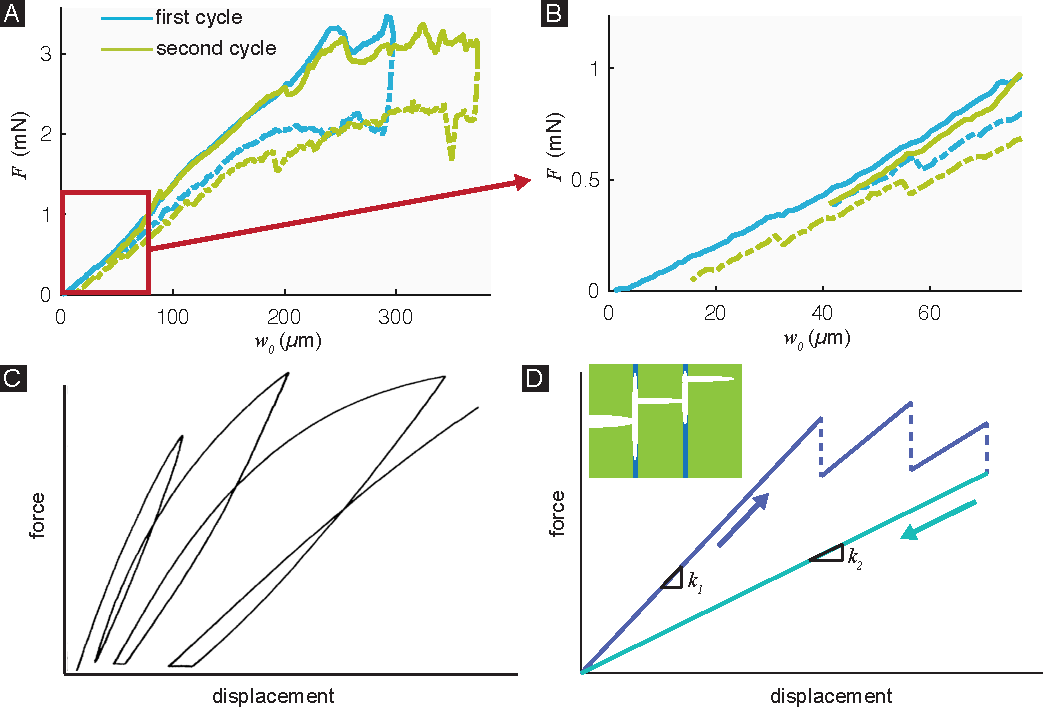
\includegraphics[width=\textwidth]{Figures/Figure6_V3.pdf}
\caption{Force-displacement response from simply-supported load-unload tests. (\textsf{A}) A representative $F$-$w_0$ response of an \EA spicule that was subjected to two load-unload cycles in the simply-supported setup. The blue and green
%, green, and yellow
curves correspond to the first and second
%, second and third
load-unload cycles, respectively. The solid portion of each curve corresponds to the loading branch and the dashed section corresponds to the unloading branch. (\textsf{B}) A zoomed in view of the plot region within the red rectangle from (\textsf{A}). (\textsf{C}) The force-displacement response of nacre from \textit{Pinctada margaritifera} in cyclic load-unload tests in a three-point bending setup (reprinted with permission from~\cite{currey1977mechanical}). (\textsf{D}) A schematic representation of the $F$ vs. $w_0$ curve of a material that experiences a sequence of crack extension and deflection events. The inset is a schematic depicting crack growth, arrest, and deflection in the material (green) that contains thin interlayers (blue). The dotted lines indicate drop in the force that correspond to unstable crack growth but not catastrophic failure. Upon unloading, the stiffness $k_2$ of the damaged specimen would be less than the stiffness $k_1$ of the undamaged specimen~\cite{ouchterlony1981extension,bush1976experimentally}.}
\label{fig:TPBcyclic}
\end{figure}
